% Options for packages loaded elsewhere
\PassOptionsToPackage{unicode}{hyperref}
\PassOptionsToPackage{hyphens}{url}
%
\documentclass[
]{article}
\usepackage{amsmath,amssymb}
\usepackage{lmodern}
\usepackage{iftex}
\ifPDFTeX
  \usepackage[T1]{fontenc}
  \usepackage[utf8]{inputenc}
  \usepackage{textcomp} % provide euro and other symbols
\else % if luatex or xetex
  \usepackage{unicode-math}
  \defaultfontfeatures{Scale=MatchLowercase}
  \defaultfontfeatures[\rmfamily]{Ligatures=TeX,Scale=1}
\fi
% Use upquote if available, for straight quotes in verbatim environments
\IfFileExists{upquote.sty}{\usepackage{upquote}}{}
\IfFileExists{microtype.sty}{% use microtype if available
  \usepackage[]{microtype}
  \UseMicrotypeSet[protrusion]{basicmath} % disable protrusion for tt fonts
}{}
\makeatletter
\@ifundefined{KOMAClassName}{% if non-KOMA class
  \IfFileExists{parskip.sty}{%
    \usepackage{parskip}
  }{% else
    \setlength{\parindent}{0pt}
    \setlength{\parskip}{6pt plus 2pt minus 1pt}}
}{% if KOMA class
  \KOMAoptions{parskip=half}}
\makeatother
\usepackage{xcolor}
\IfFileExists{xurl.sty}{\usepackage{xurl}}{} % add URL line breaks if available
\IfFileExists{bookmark.sty}{\usepackage{bookmark}}{\usepackage{hyperref}}
\hypersetup{
  pdftitle={Phonology of T'ap'anta Abaza: examples from Inzhig-Chkun and Gumlokt},
  hidelinks,
  pdfcreator={LaTeX via pandoc}}
\urlstyle{same} % disable monospaced font for URLs
\usepackage[margin=1in]{geometry}
\usepackage{graphicx}
\makeatletter
\def\maxwidth{\ifdim\Gin@nat@width>\linewidth\linewidth\else\Gin@nat@width\fi}
\def\maxheight{\ifdim\Gin@nat@height>\textheight\textheight\else\Gin@nat@height\fi}
\makeatother
% Scale images if necessary, so that they will not overflow the page
% margins by default, and it is still possible to overwrite the defaults
% using explicit options in \includegraphics[width, height, ...]{}
\setkeys{Gin}{width=\maxwidth,height=\maxheight,keepaspectratio}
% Set default figure placement to htbp
\makeatletter
\def\fps@figure{htbp}
\makeatother
\setlength{\emergencystretch}{3em} % prevent overfull lines
\providecommand{\tightlist}{%
  \setlength{\itemsep}{0pt}\setlength{\parskip}{0pt}}
\setcounter{secnumdepth}{5}
\newlength{\cslhangindent}
\setlength{\cslhangindent}{1.5em}
\newlength{\csllabelwidth}
\setlength{\csllabelwidth}{3em}
\newlength{\cslentryspacingunit} % times entry-spacing
\setlength{\cslentryspacingunit}{\parskip}
\newenvironment{CSLReferences}[2] % #1 hanging-ident, #2 entry spacing
 {% don't indent paragraphs
  \setlength{\parindent}{0pt}
  % turn on hanging indent if param 1 is 1
  \ifodd #1
  \let\oldpar\par
  \def\par{\hangindent=\cslhangindent\oldpar}
  \fi
  % set entry spacing
  \setlength{\parskip}{#2\cslentryspacingunit}
 }%
 {}
\usepackage{calc}
\newcommand{\CSLBlock}[1]{#1\hfill\break}
\newcommand{\CSLLeftMargin}[1]{\parbox[t]{\csllabelwidth}{#1}}
\newcommand{\CSLRightInline}[1]{\parbox[t]{\linewidth - \csllabelwidth}{#1}\break}
\newcommand{\CSLIndent}[1]{\hspace{\cslhangindent}#1}
\usepackage{fontspec}
\setmainfont{Brill}
\setmonofont{Iosevka}
\usepackage{philex}
\usepackage{booktabs}
\usepackage{longtable}
\usepackage{array}
\usepackage{multirow}
\usepackage{wrapfig}
\usepackage{float}
\usepackage{colortbl}
\usepackage{pdflscape}
\usepackage{tabu}
\usepackage{threeparttable}
\usepackage{threeparttablex}
\usepackage[normalem]{ulem}
\usepackage{makecell}
\usepackage{xcolor}
\ifLuaTeX
  \usepackage{selnolig}  % disable illegal ligatures
\fi

\title{Phonology of T'ap'anta Abaza: examples from Inzhig-Chkun and
Gumlokt}
\author{G. Moroz, S. Kuznetsova\\
(HSE University)}
\date{2022-04-08}

\begin{document}
\maketitle

{
\setcounter{tocdepth}{2}
\tableofcontents
}
\pagebreak

\hypertarget{introduction}{%
\section{Introduction}\label{introduction}}

\hypertarget{general-information-about-abaza}{%
\subsection{General information about
Abaza}\label{general-information-about-abaza}}

In this article I describe two varieties of Tapanta dialect of Abaza
(ISO-639-3 \texttt{abq}, glottocode \texttt{abaz1241}) spoken in two
villages in the Karachay-Cherkess Republic: Inzhig-Chkun (in Abaza
/jənˈdʒəɡʲ-tʃk'ʷən/) and Krasniy Vostok (in Abaza /ɡʷəmˈlokt/). Abaza is
a language of the Abkhaz-Abaza group of Northwest Caucasian family of
languages. After the Caucasian War (1817--1864) a lot of Abaza, Abkhaz,
Ubykh and Adyghe people were forced either to resettle from higher
mountains or to immigrate to the Ottoman Empire. As a result Abaza
people were split into those who remain in Russia (mostly in the
Karachay-Cherkess Republic, see Figure \ref{fig:abaza-map} created with
\texttt{lingtypology} (Moroz 2017)) and who moved to Turkey. According
to the 2010 Russian census, there are slightly less than 38 thousand
speakers of Abaza in Russia. The exact number of speakers in other
countries, mainly in Turkey (Chirikba 2012: 21--23), is unknown. The
data analyzed in this study were collected in 2018, 2019 and 2021 during
a field trip to the villages. Even though traditionally Abaza is treated
as a separate language with two dialects T'ap'anta and Shkharawa (Genko
1955: 5--7; Tabulova 1976: 3--4; Lomthathidze 2006: 98), some of the
researches consider Abkhaz and Abaza to be a dialect continuum (e. g.
Hewitt 1979: 1; Colarusso 1988: 7--9; Chirikba 1996). However varieties
of Inzhig-Chkun and Gumlokt belong to the same dialect, those lects have
their own differences, e. g. \emph{Abaza language} is /abaza
bəz\textbf{ŝ}a/ in Inzhig-Chkun and /abaza bəz\textbf{ʂ}a/ in Gumlokt.

\begin{figure}

{\centering 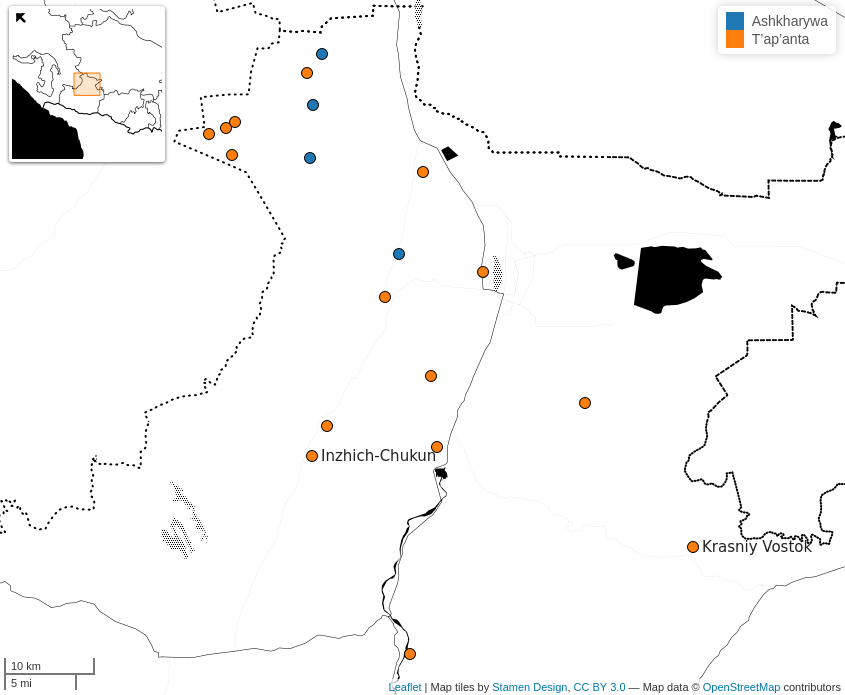
\includegraphics[width=4.22in]{images/01_abaza_map} 

}

\caption{Abaza settlements of the Karachay-Cherkess Republic colored by the dialect (mostly based on (Chirikba 2020)). In Abazakt, Adyge-Khabl, Ersakon, Khumara, and Psauche-Dakhe Circassians are predominant. In Koydan Karachay are predominant.}\label{fig:abaza-map}
\end{figure}

\hypertarget{state-of-research}{%
\subsection{State of research}\label{state-of-research}}

Phonological inventory of Abaza can be found in multiple sources (Bouda
1940; Lomthathidze 1944, 2006; Genko 1955; Allen 1956; Tabulova 1976;
Colarusso 1988; O'Herin 1992, 2021; Chirikba 1996; Arkadiev 2019),
however more detailed phonological description is limited to (Bouda
1940; Lomthathidze 1944; Genko 1955; Catford 1972; Tabulova 1976;
Colarusso 1988; Arkadiev 2019) and lack any acoustic analysis that
appears just recently (Mamonova, Moroz 2019). It is also worth
mentioning works by V. Chirikba (Chirikba 1985, 2020), where he provides
data from huge amount of Abaza settlements, explores correspondences of
post-alveolar sibilants among them and compare obtained data with data
from Abkhaz and Adyghe.

\hypertarget{phonological-inventory}{%
\section{Phonological inventory}\label{phonological-inventory}}

\hypertarget{consonants}{%
\subsection{Consonants}\label{consonants}}

Phonological inventory of T'ap'anta is present in Table
\ref{tab:phon-system}. I illustrate\footnote{In this work I will use two
  transcription systems. First system is my interpretation of Abaza
  phonology using IPA. Second is standard Abaza orthography. The IPA
  transcription used in this work differ from traditional Caucasian
  transcription, however Northwest Caucasian researchers still can
  retrieve desired information from orthographic correspondences.
  Unfortunately IPA alphabet still allows a lot of space for
  interpretation, so my system is differ from other recent phonological
  phonetic discriptions illustration of Northwest Caucasian languages
  (see (Gordon, Applebaum 2006; Andersson, Vaux, Pysipa (Şener) 2021)).
  I refuse to use symbols like ʃ, ʒ, ɕ or ʑ one can find in the
  literature for special post-alveolars sounds present in all Northwest
  Caucasian and continue to use symbols ŝ and ẑ after the following
  sources (Ladefoged, Maddieson 1996: 161--164; Catford 1997; Testelets
  et al. 2009; Applebaum, Gordon 2011; Paschen 2015).
  \label{trans-system}} consonant inventory with some examples in
Appendix 1.

\begin{table}[H]

\caption{\label{tab:phon-system}Joint consonant system of Inzhig-Chkun and Gumlokt. Parenthesis denote the system that is common for Gumlokt, where the vast mojority of speakers use labialised post-alveolar segments.}
\centering
\resizebox{\linewidth}{!}{
\begin{tabular}[t]{l|c|c|c|c|c|c|c|c|c|c|c|c}
\hline
\rotatebox{-90}{ } & \rotatebox{-90}{aspirated plosives} & \rotatebox{-90}{ejective plosives} & \rotatebox{-90}{voiced plosives} & \rotatebox{-90}{voiceless affricates} & \rotatebox{-90}{ejective affricates} & \rotatebox{-90}{voiced affricates} & \rotatebox{-90}{voiceless fricatives} & \rotatebox{-90}{voiced fricatives} & \rotatebox{-90}{nasals} & \rotatebox{-90}{approximant} & \rotatebox{-90}{tap} & \rotatebox{-90}{laterals}\\
\hline
labial & pʰ & p’ & b &  &  &  & f & v & m & w &  & \\
\hline
dental & tʰ & t’ & d & ts & ts’ & dz & s & z & n &  &  & \\
\hline
alveolar &  &  &  &  &  &  &  &  &  &  & ɾ & \\
\hline
post-alveolar (labialized) &  &  &  & tŝ(ʷ) & tŝ’(ʷ) & dẑ(ʷ) & ŝ(ʷ) & ẑ(ʷ) &  &  &  & \\
\hline
retroflex &  &  &  & tʂ & tʂ’ & dʐ & ʂ & ʐ &  &  &  & \\
\hline
alveolo-palatal &  &  &  & tɕ & tɕ’ & dʑ & ɕ & ʑ &  &  &  & \\
\hline
lateral &  &  &  &  &  &  &  &  &  &  &  & l lʲ\\
\hline
palatal & cʰ & c’ & ɟ &  &  &  & ç &  &  & j &  & \\
\hline
plain velar & kʰ & k’ & ɡ &  &  &  &  &  &  &  &  & \\
\hline
labialized velar & kʰʷ & k’ʷ & ɡʷ &  &  &  & xʷ &  &  &  &  & \\
\hline
plain uvular & qʰ & q’ &  &  &  &  & χ & ʁ &  &  &  & \\
\hline
palatalized uvular &  & q’ʲ &  &  &  &  & χʲ & ʁʲ &  &  &  & \\
\hline
labialized uvular & qʰʷ & q’ʷ &  &  &  &  & χʷ & ʁʷ &  &  &  & \\
\hline
plain pharyngeal &  &  &  &  &  &  & ħ & ʕ &  &  &  & \\
\hline
labialized pharyngeal &  &  &  &  &  &  & ħʷ & ʕʷ &  &  &  & \\
\hline
glottal &  & ʔ &  &  &  &  &  &  &  &  &  & \\
\hline
\end{tabular}}
\end{table}

The main difference between Inzhig-Chkun and Gumlokt consonant systems
is in post-alveolar consonants. All speakers of Inzhig-Chkun and some
minority in Gumlokt use non-labialized post-alveolars (e. g. ŝ, see
Figure \ref{fig:sibilants-d28}). The majority of speakers in Gumlokt use
labialised post-alveolars (e. g. ŝʷ). Everything become even more
complicated, since some post-alveolars in Inzhig-Chkun correspond to
retroflex segments in Gumlokt. It looks like there is some
proto-phonemes that merged together in most Abaza dialects except
Gumlokt and Apsua (Ashkharywa dialect, (Lomthathidze 2006: 47,
445--446)): in Apsua in the same position labialized retroflex
fricatives are observed (cf.~\ref{sh}--\ref{zh}).

\lb{sh}{ ŝə (Inzhig-Chkun), ʂə (Gumlokt), ʂʷə (Apsua) --- 'door'}
\lb{zh}{ ẑə (Inzhig-Chkun), ʐə (Gumlokt), ʐʷə (Apsua) --- 'old'}

\begin{figure}

{\centering 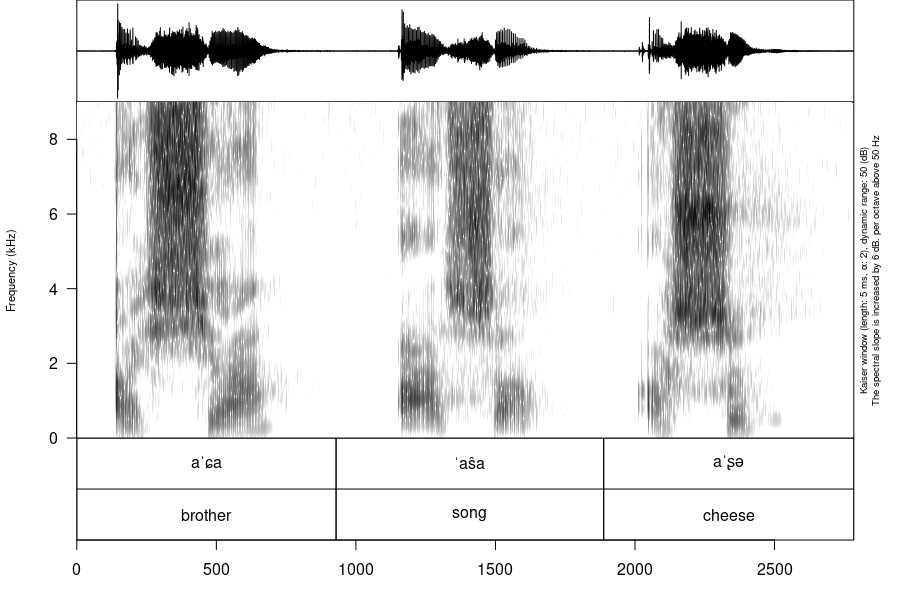
\includegraphics[width=6in]{images/03_d28_fricatives} 

}

\caption{Fricatives by female speaker with non-labialised post-alveolars.}\label{fig:sibilants-d28}
\end{figure}

Presented examples show that the post-alveolar correspondences between
Inzhig-Chkun and Gumlokt not predictable without Gumlokt or Apsua data
(see Table \ref{tab:post_alveolar}), so I decided to collect some
lexicon that could be useful for further historical and dialectal
investigation (see Appendix 2).

\begin{table}[H]

\caption{\label{tab:post_alveolar}Post-alveolar correspondences between Inzhig-Chkun and Gumlokt.}
\centering
\resizebox{\linewidth}{!}{
\begin{tabular}[t]{l|c|c|c|c}
\hline
  & Inzhig-Chkun & minority in Gumlokt & majority in Gumlokt & orthography\\
\hline
bullock & tŝə & tŝə & tŝʷə & чвы\\
\hline
apple & tŝ'a & tŝ'a & tŝ'ʷa & чIва\\
\hline
one person & zaˈdẑə & zaˈdẑə & zaˈdẑʷə & заджвы́\\
\hline
you (2pl) & ŝaˈɾa & ŝaˈɾa & ŝʷaˈɾa & швара́\\
\hline
cow & ẑə & ẑə & ẑʷə & жвы\\
\hline
hay & tŝa & tʂa & tʂa & чва́\\
\hline
oak & dʑtŝ’ə & dʑtʂ’ə & dʑtʂ’ə & джьчIвы\\
\hline
to go out & wˈdẑəlts’ & wˈdʐəlts’ & wˈdʐəlts’ & уджвы́лцI\\
\hline
door & ŝə & ʂə & ʂə & швы\\
\hline
old & ẑə & ʐə & ʐə & жвы\\
\hline
\end{tabular}}
\end{table}

It is worth mentioning that in (Chirikba 2020) based on different
resources Vyacheslav Chirikba discovered even bigger variation. There
are four sibilant subsystems in (ibid.: 27), however our field data
support only two types: with labialised post-alveolars (majority) and
with non-labialised post-alveolars (minority). In order to check my
hypothesis I performed small experiment asking 31 Gumlokt speakers (15
female and 16 male speakers) for two words: ẑ(ʷ)ə `cow' and tŝ`(ʷ)a
'apple'. As I found indeed there is a variation across speakers I worked
with, however only Gumlokt 2 (with labialised post-alveolars, 25 people)
and Gumlokt 1 (with non-labialised post-alveolars, 6 people) sibilant
subsytems from (ibid.) were attested (see Figure
\ref{fig:experiment-results}). It also visible from the experiment
results that non-labialised post-alveolars are tend to appear in speach
of older females, but this is just a preliminary result that should be
checked with greater number of stimuli and speakers.

\begin{figure}

{\centering 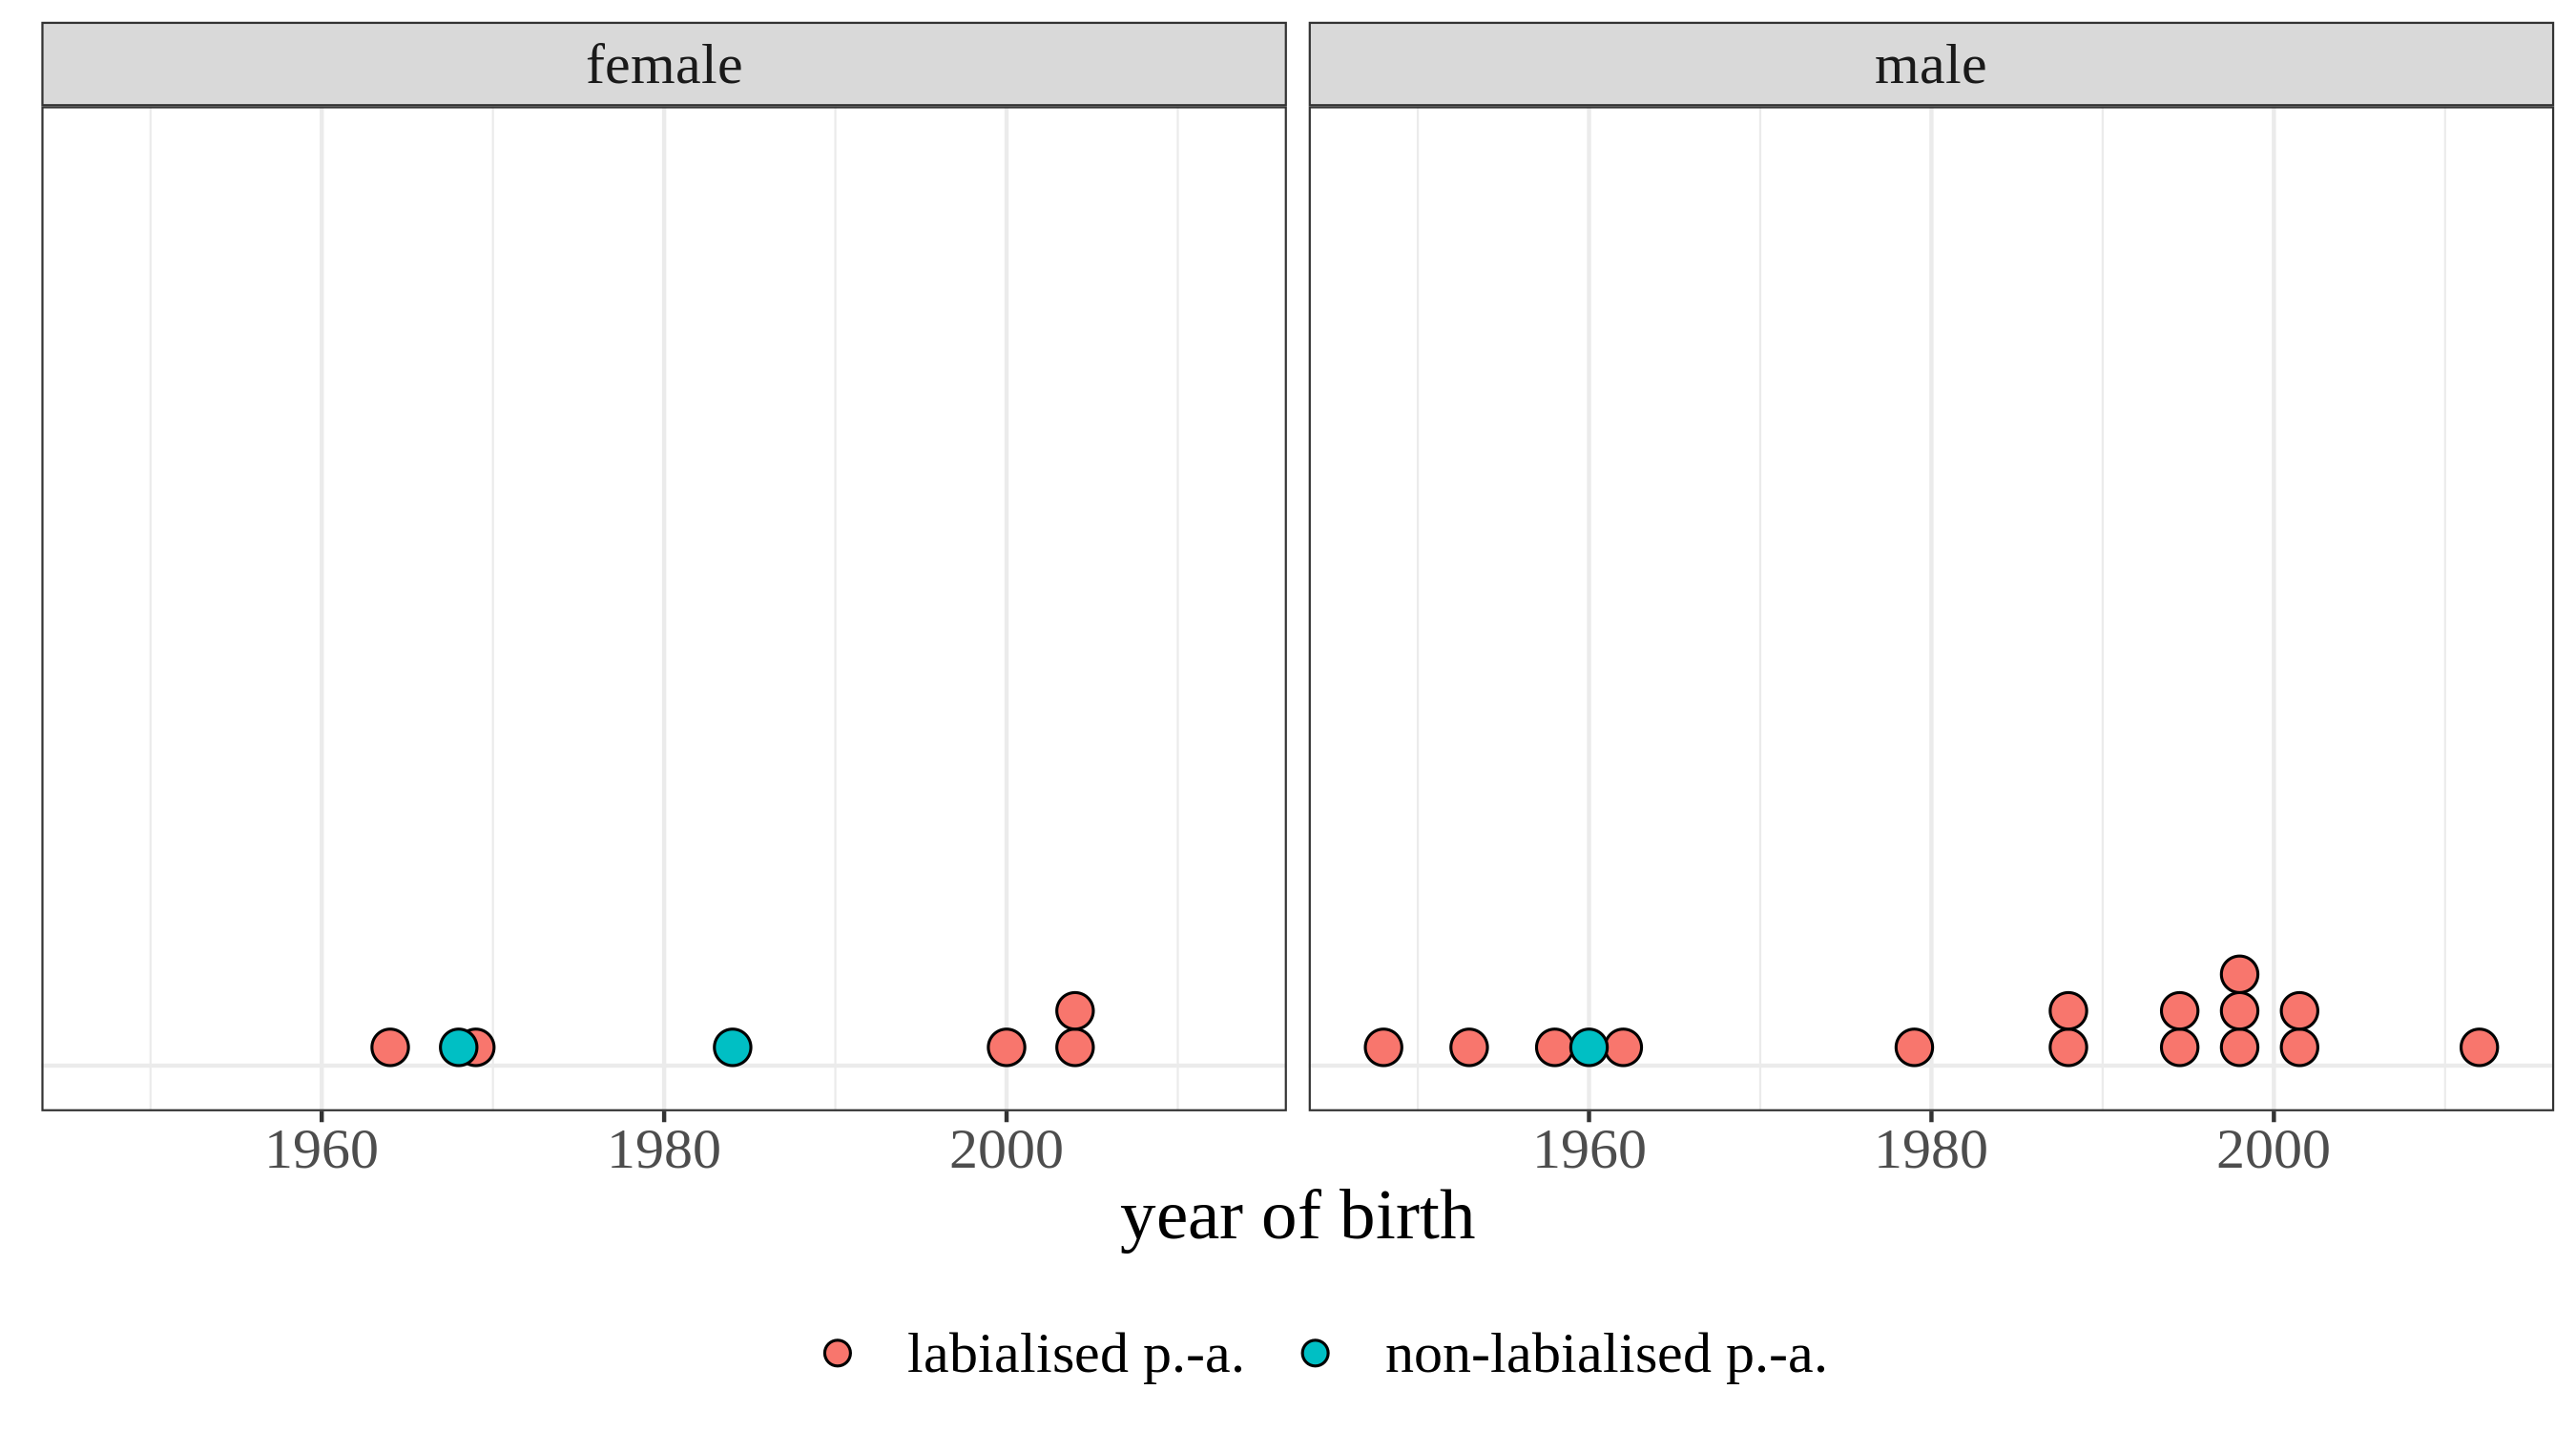
\includegraphics[width=5.4in]{images/02_experiment} 

}

\caption{Results of experiment. Each dot represents one person colored by result and faceted by gender.}\label{fig:experiment-results}
\end{figure}

Except of my interpretation of alveolar and retroflex consonants (see
the footnote on the page \pageref{trans-system}) the main difference
between my phonological description and older ones is in the palatal
area: I treat segments cʰ, c', and ɟ as palatal, however more
traditional interpretation is palatalized velars: kʲ, k', and ɡʲ.

Articulation of labialization in T'ap'anta is different for different
places of articulation (see (Catford 1972) for the similar observations
for Abkhaz):

\begin{itemize}
\tightlist
\item
  /w/-labialisation --- this kind of labialization is more or less
  independent of the main place of articulation. This kind of
  labialisation is typical for velar and uvular places fricatives and
  stops;
\item
  /ɥ/-labialisation --- this kind of labialization is typical for
  pharyngeals. It looks like the tongue body is retracted (due to
  pharyngeal place of articulation) and raised, that results /ɥ/-like
  sound;
\item
  /y/-labialisation --- this kind of labialization is typical only for
  post-alveolars in Gumlokt. The main place of articulation somehow
  merged with the additional place of articulation that produces a long
  hole for /y/-like sound.
\end{itemize}

There is also so called weaken labialised post-alveolars mentioned in
literature (Chirikba 1985, 2020; Lomthathidze 1944), but we didn't
noticed such sounds neither in Inzhig-Chkun nor Gumlokt.

\hypertarget{vowels}{%
\subsection{Vowels}\label{vowels}}

The vowel inventory traditionally analized as two core vowels a (low)
and ə (mid) (see (Bouda 1940; Lomthathidze 1944, 2006; Genko 1955; Allen
1956; Tabulova 1976; Colarusso 1988; O'Herin 1992, 2021; Chirikba 1996;
Arkadiev 2019)). There are additional vowel colors that appear in
numerous loanwords or due to contraction of vowel and glide
(cf.~\ref{i}--\ref{o}):

\lb{i}{ i < əj or jə;}
\lb{e}{ e < aj;}
\lb{u}{ u < əw or wə;}
\lb{o}{ o < aw.}

In order to show vowel space I collected a list of monosyllabic words in
Inzhig-Chkun and Gumlokt (see Appendix 3).

\hypertarget{stress}{%
\section{Stress}\label{stress}}

T'ap'anta Abaza stress was discussed in my unpublished report from
previous expeditions and became a basis for (Arkadiev 2019).
Unfortunately I've changed my opinion, so I will try to sum up my
current opinion on the topic. Our stress model based on the ideas
presented in (Dybo 1977; Spruit 1986).

Stress in Abaza is distinctive (see (\ref{stress}) and other examples in
Appendix 4).

\lb{stress}{ saˈɾa 'I' vs. ˈsaɾa 'lamb'}

Each Abaza morpheme (even borrowed) can be represented by combination of
open syllables with vowel a or ə. According to some test discussed
bellow each syllable assigned to one of the accentual classes: dominant
or recessive. The main stress rule is formulated in (Spruit 1986:
37--40): stress falls on the first D element followed by R or word
boundary (see () and \ldots), otherwise stress is on the first syllable
(see \ldots).

\pagebreak

\hypertarget{appendix-1-list-of-consonant-examples}{%
\section*{Appendix 1: List of consonant
examples}\label{appendix-1-list-of-consonant-examples}}
\addcontentsline{toc}{section}{Appendix 1: List of consonant examples}

Example words for consonants from Table \ref{tab:phon-system}. First
example before slash is from Inzhig-Chkun and some speakers from
Gumlokt, example after slash are common for most speakers from Gumlokt.

\begin{longtable}{l|l|l}
\hline
transcription & orthography & translation\\
\hline
\endfirsthead
\multicolumn{3}{@{}l}{}\\
\hline
transcription & orthography & translation\\
\hline
\endhead
\cellcolor{gray!6}{pʰa} & \cellcolor{gray!6}{па} & \cellcolor{gray!6}{son}\\
\hline
p’aj & пIай & dirt\\
\hline
\cellcolor{gray!6}{ba} & \cellcolor{gray!6}{ба} & \cellcolor{gray!6}{you (2sgf)}\\
\hline
faˈɾa & фара́ & to eat\\
\hline
\cellcolor{gray!6}{ma} & \cellcolor{gray!6}{ма} & \cellcolor{gray!6}{here you are (giving something)}\\
\hline
wa & уа & you (2sgm)\\
\hline
\cellcolor{gray!6}{ˈtʰaba} & \cellcolor{gray!6}{та́ба} & \cellcolor{gray!6}{frying pan}\\
\hline
ˈt’at’a & тIа́тIа & soft\\
\hline
\cellcolor{gray!6}{da} & \cellcolor{gray!6}{да} & \cellcolor{gray!6}{tendon}\\
\hline
tsa & ца & barn\\
\hline
\cellcolor{gray!6}{ts’a} & \cellcolor{gray!6}{цIа} & \cellcolor{gray!6}{louse}\\
\hline
dza & дза & rib\\
\hline
\cellcolor{gray!6}{sa} & \cellcolor{gray!6}{са} & \cellcolor{gray!6}{I}\\
\hline
ˈʕʷaza & гIва́за & twins\\
\hline
\cellcolor{gray!6}{naˈʕa} & \cellcolor{gray!6}{нагIа́} & \cellcolor{gray!6}{slope}\\
\hline
baˈɾa & бара́ & you (2sgf)\\
\hline
\cellcolor{gray!6}{tŝa / tŝʷa} & \cellcolor{gray!6}{чва} & \cellcolor{gray!6}{skin}\\
\hline
tŝ’a / tŝ’ʷa & чIва & apple\\
\hline
\cellcolor{gray!6}{dẑaˈɾa / dẑʷaˈɾa} & \cellcolor{gray!6}{джвара́} & \cellcolor{gray!6}{vomiting}\\
\hline
ŝa / ŝʷa & шва & you (2pl)\\
\hline
\cellcolor{gray!6}{aˈẑa / aˈẑʷa} & \cellcolor{gray!6}{ажва́} & \cellcolor{gray!6}{word}\\
\hline
ˈtʂaba & тша́ба & gelding\\
\hline
\cellcolor{gray!6}{tʂ’a} & \cellcolor{gray!6}{шIа} & \cellcolor{gray!6}{mouth}\\
\hline
ˈpʰadʐa & па́джа & firstborn\\
\hline
\cellcolor{gray!6}{ʂaˈba} & \cellcolor{gray!6}{шаба́} & \cellcolor{gray!6}{dried-up}\\
\hline
ˈʐac’a & жа́кIьа & beard\\
\hline
\cellcolor{gray!6}{tɕaˈɾa} & \cellcolor{gray!6}{чара́} & \cellcolor{gray!6}{to eat}\\
\hline
ˈtɕ’atɕ’a & чIа́чIа & kidney\\
\hline
\cellcolor{gray!6}{ˈdʑadʑa} & \cellcolor{gray!6}{джьа́джьа} & \cellcolor{gray!6}{curly}\\
\hline
ɕa & ща & blood\\
\hline
\cellcolor{gray!6}{ʑaˈɾa} & \cellcolor{gray!6}{жьара́} & \cellcolor{gray!6}{to deceive}\\
\hline
la & ла & dog\\
\hline
\cellcolor{gray!6}{lʲaˈɡʲan} & \cellcolor{gray!6}{льагьан} & \cellcolor{gray!6}{basin}\\
\hline
ˈmacʰa & ма́кьа & grindstone\\
\hline
\cellcolor{gray!6}{ˈc’ana} & \cellcolor{gray!6}{кIьа́на} & \cellcolor{gray!6}{lump}\\
\hline
ˈɟaba & гьа́ба & (body) side\\
\hline
\cellcolor{gray!6}{ˈçapʰad} & \cellcolor{gray!6}{тлапа́д} & \cellcolor{gray!6}{stocking}\\
\hline
jaˈɾa & йара́ & he (3sgm)\\
\hline
\cellcolor{gray!6}{kʰətʰ} & \cellcolor{gray!6}{кыт} & \cellcolor{gray!6}{village}\\
\hline
k’aˈɾa & кIара́ & something\\
\hline
\cellcolor{gray!6}{ˈɡaɾa} & \cellcolor{gray!6}{га́ра} & \cellcolor{gray!6}{cradle}\\
\hline
kʰʷa & ква & rain\\
\hline
\cellcolor{gray!6}{k’ʷa} & \cellcolor{gray!6}{кIва} & \cellcolor{gray!6}{bosom}\\
\hline
ɡʷaˈban & гваба́н & mattress\\
\hline
\cellcolor{gray!6}{ˈxʷatʰa} & \cellcolor{gray!6}{хва́та} & \cellcolor{gray!6}{rug}\\
\hline
qʰa & хъа & head\\
\hline
\cellcolor{gray!6}{q’aˈla} & \cellcolor{gray!6}{къала́} & \cellcolor{gray!6}{town}\\
\hline
χaˈɾa & хара́ & to give a present\\
\hline
\cellcolor{gray!6}{ˈʁaʁa} & \cellcolor{gray!6}{гъа́гъа} & \cellcolor{gray!6}{broad, wide}\\
\hline
ˈq’ʲaɾa & къьара́ & to wave\\
\hline
\cellcolor{gray!6}{χʲaˈɾa} & \cellcolor{gray!6}{хьара́} & \cellcolor{gray!6}{to give birth}\\
\hline
ʁʲaˈsa & гъьаса́ & nutwood\\
\hline
\cellcolor{gray!6}{qʰʷa} & \cellcolor{gray!6}{хъва} & \cellcolor{gray!6}{ashes}\\
\hline
q’ʷaˈɾa & къвара́ & to stay too long\\
\hline
\cellcolor{gray!6}{χʷa} & \cellcolor{gray!6}{хва} & \cellcolor{gray!6}{mountain}\\
\hline
tŝʷaˈʁʷa & чвагъва́ & ploughed up\\
\hline
\cellcolor{gray!6}{ħa} & \cellcolor{gray!6}{хIа} & \cellcolor{gray!6}{we}\\
\hline
aˈʕa & агIа́ & raw leather\\
\hline
\cellcolor{gray!6}{ħʷa} & \cellcolor{gray!6}{хIва} & \cellcolor{gray!6}{pig}\\
\hline
ʕʷa & гIва & dry\\
\hline
\cellcolor{gray!6}{aˈʔaɕa} & \cellcolor{gray!6}{аъа́ща} & \cellcolor{gray!6}{situation}\\
\hline
\end{longtable}

\pagebreak

\hypertarget{appendix-2-post-alveolarretroflex-correspondences-to-inzhig-chkuns-post-alveolars-in-gumlokt}{%
\section*{Appendix 2: Post-alveolar/retroflex correspondences to
Inzhig-Chkun's post-alveolars in
Gumlokt}\label{appendix-2-post-alveolarretroflex-correspondences-to-inzhig-chkuns-post-alveolars-in-gumlokt}}
\addcontentsline{toc}{section}{Appendix 2: Post-alveolar/retroflex
correspondences to Inzhig-Chkun's post-alveolars in Gumlokt}

\begin{longtable}{l|l|l}
\hline
transcription & orthography & translation\\
\hline
\endfirsthead
\multicolumn{3}{@{}l}{}\\
\hline
transcription & orthography & translation\\
\hline
\endhead
\cellcolor{gray!6}{zaˈdẑʷə} & \cellcolor{gray!6}{заджвы́} & \cellcolor{gray!6}{one person}\\
\hline
dẑʷdẑʷə & джвджвы & saliva\\
\hline
\cellcolor{gray!6}{ħadẑʷ} & \cellcolor{gray!6}{хIаджв} & \cellcolor{gray!6}{stack}\\
\hline
ŝʷaˈɾa & швара́ & you\\
\hline
\cellcolor{gray!6}{alaɾŝʷaˈɾa} & \cellcolor{gray!6}{аларшвара́} & \cellcolor{gray!6}{to turn on}\\
\hline
ˈaŝʷa & а́шва & song\\
\hline
\cellcolor{gray!6}{ɡʷlaŝʷ} & \cellcolor{gray!6}{гвлашв} & \cellcolor{gray!6}{indifferent}\\
\hline
ˈɟaŝʷa & гьа́шва & orphaned\\
\hline
\cellcolor{gray!6}{k’aŝʷaˈɾa} & \cellcolor{gray!6}{кIашвара́} & \cellcolor{gray!6}{to fall}\\
\hline
kʷɾəŝʷ & кврышв & patch\\
\hline
\cellcolor{gray!6}{laŝʷ} & \cellcolor{gray!6}{лашв} & \cellcolor{gray!6}{blind}\\
\hline
maɾatʰaˈŝʷaɾtʰa & мараташва́рта & west\\
\hline
\cellcolor{gray!6}{nabˈʁaŝʷ} & \cellcolor{gray!6}{набгъа́шв} & \cellcolor{gray!6}{one year old foal}\\
\hline
pʰəŝʷtʰ amamk’ʷa & пышвт ама́мкIва & without break\\
\hline
\cellcolor{gray!6}{wəˈdzəŝʷa} & \cellcolor{gray!6}{удзыш́ва} & \cellcolor{gray!6}{green}\\
\hline
wəˈnaŝʷa & уна́шва & advice\\
\hline
\cellcolor{gray!6}{qʰŝʷa} & \cellcolor{gray!6}{хъвшва} & \cellcolor{gray!6}{food (cooked)}\\
\hline
ts’aˈŝʷa & цIашва́ & trump card\\
\hline
\cellcolor{gray!6}{ˈŝʷabəʐ} & \cellcolor{gray!6}{шва́быж} & \cellcolor{gray!6}{very}\\
\hline
ˈŝʷapχa & шва́пха & example\\
\hline
\cellcolor{gray!6}{ˈŝʷaχʲa} & \cellcolor{gray!6}{швахьа́} & \cellcolor{gray!6}{Monday}\\
\hline
ŝʷwocʰ & швуокь & gun\\
\hline
\cellcolor{gray!6}{ŝʷəɾ} & \cellcolor{gray!6}{швыр} & \cellcolor{gray!6}{fruit}\\
\hline
ʂə & шы & door\\
\hline
\cellcolor{gray!6}{aˈʂə} & \cellcolor{gray!6}{ашы́} & \cellcolor{gray!6}{cheese}\\
\hline
ajˈʂa & айша́ & traditional table\\
\hline
\cellcolor{gray!6}{ˈajʂa} & \cellcolor{gray!6}{а́йша} & \cellcolor{gray!6}{bitter}\\
\hline
bʐaˈʂə & бжашы́ & not fully painted\\
\hline
\cellcolor{gray!6}{ʂk’ə} & \cellcolor{gray!6}{шкIы} & \cellcolor{gray!6}{hundred}\\
\hline
bəzˈʂa & бызша́ & language\\
\hline
\cellcolor{gray!6}{ɡʷaʂ} & \cellcolor{gray!6}{гваш} & \cellcolor{gray!6}{gate}\\
\hline
laˈʂan & лаша́н & time for weeding\\
\hline
\cellcolor{gray!6}{mʂə} & \cellcolor{gray!6}{мшы} & \cellcolor{gray!6}{bear}\\
\hline
ɾʂaˈɾa & ршара́ & to scare\\
\hline
\cellcolor{gray!6}{nəʂ} & \cellcolor{gray!6}{ныш} & \cellcolor{gray!6}{clay}\\
\hline
tʰaɾaʂ & тара́ш & gate\\
\hline
\cellcolor{gray!6}{qʰʷʂə} & \cellcolor{gray!6}{хъвшы} & \cellcolor{gray!6}{medicine}\\
\hline
qʰəʂ & хъыш & window\\
\hline
\cellcolor{gray!6}{tɕaʂ} & \cellcolor{gray!6}{чаш} & \cellcolor{gray!6}{patty}\\
\hline
ʂaˈʕʷə & шагIвы́ & fearful\\
\hline
\cellcolor{gray!6}{ʂaɡaˈla} & \cellcolor{gray!6}{шагала́} & \cellcolor{gray!6}{pack of jackal}\\
\hline
ʂp’a & шпIа & thick\\
\hline
\cellcolor{gray!6}{ʂʔa} & \cellcolor{gray!6}{шъа} & \cellcolor{gray!6}{document}\\
\hline
ʂəɾ & шыр & animal\\
\hline
\cellcolor{gray!6}{tŝ’ʷa} & \cellcolor{gray!6}{чIва} & \cellcolor{gray!6}{apple}\\
\hline
amts’tŝ’ʷaˈɾa & амцIчIвара́ & to rob\\
\hline
\cellcolor{gray!6}{aˈqʰatŝʷɾa} & \cellcolor{gray!6}{ахъа́чIвра} & \cellcolor{gray!6}{to stitch}\\
\hline
jaˈtŝʷa & йачIва́ & star\\
\hline
\cellcolor{gray!6}{jaˈtŝ’ʷa} & \cellcolor{gray!6}{йачIва́} & \cellcolor{gray!6}{grey}\\
\hline
kʷajˈtŝ’ʷa & квайчIва́ & black\\
\hline
\cellcolor{gray!6}{mətʂ’ʷ} & \cellcolor{gray!6}{мычIв} & \cellcolor{gray!6}{shy}\\
\hline
pʰətŝ’ʷ & пычIв & initial\\
\hline
\cellcolor{gray!6}{waˈtŝ’ʷə} & \cellcolor{gray!6}{уачIвы́} & \cellcolor{gray!6}{tomorrow}\\
\hline
tŝ’ʷɾa & чIвра & to turn sour\\
\hline
\cellcolor{gray!6}{tŝ’ʷə} & \cellcolor{gray!6}{чIвы} & \cellcolor{gray!6}{bolt}\\
\hline
tŝʷə & чвы & bullock\\
\hline
\cellcolor{gray!6}{ˈtŝʷaẑʷaɾa} & \cellcolor{gray!6}{чва́жвара} & \cellcolor{gray!6}{to \vphantom{1} speak}\\
\hline
anˈtŝʷaʑ & анчва́жь & birthmark\\
\hline
\cellcolor{gray!6}{ˈaqʰatŝʷaɕaɾa} & \cellcolor{gray!6}{а́хъачващара} & \cellcolor{gray!6}{to find respectable}\\
\hline
aˈtŝʷədzɾa & ачвы́дзра & to lose something\\
\hline
\cellcolor{gray!6}{bnatŝʷ} & \cellcolor{gray!6}{бначв} & \cellcolor{gray!6}{aurochs}\\
\hline
tŝʷa & чва & \vphantom{1} skin\\
\hline
\cellcolor{gray!6}{tŝʷɾa} & \cellcolor{gray!6}{чвра} & \cellcolor{gray!6}{to cut (wood)}\\
\hline
tŝʷa & чва & color\\
\hline
\cellcolor{gray!6}{dzətŝʷ} & \cellcolor{gray!6}{дзычва} & \cellcolor{gray!6}{swan}\\
\hline
ẑʷtŝʷa & жвчва & overdone (about \vphantom{1} food)\\
\hline
\cellcolor{gray!6}{ˈq’ətŝʷɡa} & \cellcolor{gray!6}{къы́чвга} & \cellcolor{gray!6}{hatchet}\\
\hline
maˈtŝʷə & мачвЫ & finger\\
\hline
\cellcolor{gray!6}{maˈtŝʷəsɾa} & \cellcolor{gray!6}{мачвы́сра} & \cellcolor{gray!6}{glare (about lightning)}\\
\hline
anˈtŝʷa & анчва́ & God\\
\hline
\cellcolor{gray!6}{ˈnətŝʷa} & \cellcolor{gray!6}{ны́чва} & \cellcolor{gray!6}{hemp}\\
\hline
pʰəɾtŝʷ & пы́рчв & mane\\
\hline
\cellcolor{gray!6}{ˈpʂatŝʷɟa} & \cellcolor{gray!6}{пша́чвгьа} & \cellcolor{gray!6}{strong wind}\\
\hline
tŝʷaˈɾa & чвара́ & dream\\
\hline
\cellcolor{gray!6}{tʕaˈtŝʷa, tħaˈtŝʷa} & \cellcolor{gray!6}{тгIачва́, тхIачва́} & \cellcolor{gray!6}{family}\\
\hline
qʰətŝʷ & хъы́чв & bird comb\\
\hline
\cellcolor{gray!6}{tŝʷa} & \cellcolor{gray!6}{чва} & \cellcolor{gray!6}{skin}\\
\hline
tŝʷaˈba & чваба́ & wax\\
\hline
\cellcolor{gray!6}{tŝʷaˈħʷa} & \cellcolor{gray!6}{чвахIва́} & \cellcolor{gray!6}{stripe}\\
\hline
tŝʷbza & чвбза & lover\\
\hline
\cellcolor{gray!6}{tŝʷɟa} & \cellcolor{gray!6}{чвгьа} & \cellcolor{gray!6}{evil}\\
\hline
tŝʷcʰaɕ & чвкьа́щ & shabby\\
\hline
\cellcolor{gray!6}{tŝʷts’aˈɾa} & \cellcolor{gray!6}{чвцIара́} & \cellcolor{gray!6}{to scatter}\\
\hline
tŝʷəʂ & чвыш & pale\\
\hline
\cellcolor{gray!6}{alaɾˈtʂa} & \cellcolor{gray!6}{алартшА} & \cellcolor{gray!6}{alloyed}\\
\hline
laˈtʂa & латшА & ferment\\
\hline
\cellcolor{gray!6}{maˈtʂa} & \cellcolor{gray!6}{матшА} & \cellcolor{gray!6}{dishes}\\
\hline
pslaˈtʂa & пслатша́ & fish\\
\hline
\cellcolor{gray!6}{ˈakʷtʂaɡa} & \cellcolor{gray!6}{а́квтшага} & \cellcolor{gray!6}{watering-pot}\\
\hline
tʰatʂaˈɾa & татшара́ & to pour\\
\hline
\cellcolor{gray!6}{tʂa} & \cellcolor{gray!6}{тша} & \cellcolor{gray!6}{hay}\\
\hline
atʂ’ʂaˈɾa & ашIшарА & to be afraid of\\
\hline
\cellcolor{gray!6}{ˈakʰʷtʂ’aɾa} & \cellcolor{gray!6}{а́квшIара} & \cellcolor{gray!6}{to sit down}\\
\hline
aˈtʂ’əja & ашIы́йа & what\\
\hline
\cellcolor{gray!6}{bəlˈtʂ’ə} & \cellcolor{gray!6}{былшIы́} & \cellcolor{gray!6}{fuel}\\
\hline
dʑtʂ’ə & джьшIы & oak\\
\hline
\cellcolor{gray!6}{nq’ʷɡaˈtʂ’ə} & \cellcolor{gray!6}{нкъвгашIы́} & \cellcolor{gray!6}{sick person}\\
\hline
pssʕaˈtʂ’ə & пссгIашIы́ & bird\\
\hline
\cellcolor{gray!6}{χaˈtʂ’ə} & \cellcolor{gray!6}{хашIы́} & \cellcolor{gray!6}{task}\\
\hline
ẑʷə & жвы & cow\\
\hline
\cellcolor{gray!6}{aˈẑʷa} & \cellcolor{gray!6}{ажва́} & \cellcolor{gray!6}{word}\\
\hline
baẑʷ & бажв & abundant\\
\hline
\cellcolor{gray!6}{ˈɡʷəẑʷk’ɾa} & \cellcolor{gray!6}{гвыж́вкIра} & \cellcolor{gray!6}{to be angry}\\
\hline
ẑʷba & жвба & nine\\
\hline
\cellcolor{gray!6}{ẑʷʕʷaˈqʰa} & \cellcolor{gray!6}{жвгIвахъа́} & \cellcolor{gray!6}{shoulder}\\
\hline
ẑʷʕʷa & жвгIва & cow that didn’t gave birth\\
\hline
\cellcolor{gray!6}{ẑʷʕʷand} & \cellcolor{gray!6}{жвгIванд} & \cellcolor{gray!6}{sky}\\
\hline
ẑʷp’a & жвпIа & thick\\
\hline
\cellcolor{gray!6}{ẑʷɾa} & \cellcolor{gray!6}{жвра} & \cellcolor{gray!6}{drink}\\
\hline
ẑʷts’ə & жвцIы & swallow\\
\hline
\cellcolor{gray!6}{ts’əẑʷ} & \cellcolor{gray!6}{цIыжв} & \cellcolor{gray!6}{tick}\\
\hline
χts’əẑʷ & хцIыжв & accidental bullet\\
\hline
\cellcolor{gray!6}{ˈtŝʷaẑʷaɾa} & \cellcolor{gray!6}{чва́жвара} & \cellcolor{gray!6}{to speak}\\
\hline
ˈɕaẑʷəʕʷ & ща́жвыгIв & bloodsucker\\
\hline
\cellcolor{gray!6}{pʰəẑʷˈbana} & \cellcolor{gray!6}{пыжвба́на} & \cellcolor{gray!6}{hedgehog}\\
\hline
ẑʷɾa & жвра & to boil, to drink\\
\hline
\cellcolor{gray!6}{ẑʷtŝʷa} & \cellcolor{gray!6}{жвчва} & \cellcolor{gray!6}{overdone (about food)}\\
\hline
aˈʐə & ажы & old\\
\hline
\cellcolor{gray!6}{ˈʕatʂ’ʐaɾa} & \cellcolor{gray!6}{гIа́шIжара} & \cellcolor{gray!6}{to tear off}\\
\hline
ʐaˈba & жаба́ & ten\\
\hline
\cellcolor{gray!6}{ˈʐʐaɡa} & \cellcolor{gray!6}{жжа́га} & \cellcolor{gray!6}{harrow}\\
\hline
tʰaʐ & таж & grandmother\\
\hline
\cellcolor{gray!6}{wasaˈɾaʐ} & \cellcolor{gray!6}{уасара́ж} & \cellcolor{gray!6}{wise}\\
\hline
wʐə & ужы́ & now\\
\hline
\end{longtable}

\pagebreak

\hypertarget{appendix-3-list-of-monosyllabic-words-for-the-vowel-space-research}{%
\section*{Appendix 3: List of monosyllabic words for the vowel space
research}\label{appendix-3-list-of-monosyllabic-words-for-the-vowel-space-research}}
\addcontentsline{toc}{section}{Appendix 3: List of monosyllabic words
for the vowel space research}

\begin{longtable}{l|l|l}
\hline
transcription & orthography & translation\\
\hline
\endfirsthead
\multicolumn{3}{@{}l}{}\\
\hline
transcription & orthography & translation\\
\hline
\endhead
\cellcolor{gray!6}{mʁə} & \cellcolor{gray!6}{мгъы} & \cellcolor{gray!6}{thorn}\\
\hline
mza & мза & lamp\\
\hline
\cellcolor{gray!6}{mzə} & \cellcolor{gray!6}{мзы} & \cellcolor{gray!6}{moon}\\
\hline
mzətɕ & мзыч & tree pitch\\
\hline
\cellcolor{gray!6}{mχʲæ} & \cellcolor{gray!6}{мхьа} & \cellcolor{gray!6}{sterile}\\
\hline
mtsa & мца & fire\\
\hline
\cellcolor{gray!6}{mtsə} & \cellcolor{gray!6}{мцы} & \cellcolor{gray!6}{lie}\\
\hline
mtɕɪ & мчы & strong\\
\hline
\cellcolor{gray!6}{mtʂ’tʂət} & \cellcolor{gray!6}{мшIтшыт} & \cellcolor{gray!6}{piece of wood}\\
\hline
mʂə & мшы & day\\
\hline
\cellcolor{gray!6}{mʔa} & \cellcolor{gray!6}{мъа} & \cellcolor{gray!6}{belt}\\
\hline
pʰa & па & son\\
\hline
\cellcolor{gray!6}{pʰeɕ} & \cellcolor{gray!6}{пещ} & \cellcolor{gray!6}{room}\\
\hline
sbəb & сбыб & blister\\
\hline
\cellcolor{gray!6}{psqʰa} & \cellcolor{gray!6}{псхъа} & \cellcolor{gray!6}{dead body}\\
\hline
psə & псы & soul\\
\hline
\cellcolor{gray!6}{ptʂtʂə} & \cellcolor{gray!6}{птштшы} & \cellcolor{gray!6}{broken}\\
\hline
pʰud & пуд & cheap\\
\hline
\cellcolor{gray!6}{pχa} & \cellcolor{gray!6}{пха} & \cellcolor{gray!6}{heat}\\
\hline
pχdzə & пхдзы & sweat\\
\hline
\cellcolor{gray!6}{pχtə} & \cellcolor{gray!6}{пхты} & \cellcolor{gray!6}{scab}\\
\hline
pχəz & пхыз & sleep\\
\hline
\cellcolor{gray!6}{pʂa} & \cellcolor{gray!6}{пша} & \cellcolor{gray!6}{wind}\\
\hline
pʂdza & пшдза & beautiful\\
\hline
\cellcolor{gray!6}{pʂkʰa} & \cellcolor{gray!6}{пшка} & \cellcolor{gray!6}{soft}\\
\hline
pʂəχʲ & пшыхь & breeze\\
\hline
\cellcolor{gray!6}{pɕba} & \cellcolor{gray!6}{пщба} & \cellcolor{gray!6}{four}\\
\hline
pʰədʑ & пыджь & buckle\\
\hline
\cellcolor{gray!6}{pʰəts} & \cellcolor{gray!6}{пыц} & \cellcolor{gray!6}{tooth}\\
\hline
sa & са & I\\
\hline
\cellcolor{gray!6}{skʰʷʂə} & \cellcolor{gray!6}{сквшы} & \cellcolor{gray!6}{year}\\
\hline
skʰʷʂəzcʰ & сквшызкь & thousand years\\
\hline
\cellcolor{gray!6}{ssa} & \cellcolor{gray!6}{сса} & \cellcolor{gray!6}{small}\\
\hline
staʑ & стажь & let me come down\\
\hline
\cellcolor{gray!6}{sə} & \cellcolor{gray!6}{сы} & \cellcolor{gray!6}{snow}\\
\hline
səs & сыс & lamb\\
\hline
\cellcolor{gray!6}{tc’i} & \cellcolor{gray!6}{ткIьи} & \cellcolor{gray!6}{strict}\\
\hline
tdzə & тдзы & hous\\
\hline
\cellcolor{gray!6}{tʰopʰ} & \cellcolor{gray!6}{топ} & \cellcolor{gray!6}{ball}\\
\hline
tʂbəɡ & тшбыг & scythe\\
\hline
\cellcolor{gray!6}{tʂʑɪ} & \cellcolor{gray!6}{тшжьы} & \cellcolor{gray!6}{horse meat}\\
\hline
tʂpsaχ & тшпсАх & to change (imp)\\
\hline
\cellcolor{gray!6}{tʂpɕæ} & \cellcolor{gray!6}{тшпщА} & \cellcolor{gray!6}{to rest (imp)}\\
\hline
tʂpəts & тшпыц & horse tooth\\
\hline
\cellcolor{gray!6}{tʂɾədz} & \cellcolor{gray!6}{тшрыдз} & \cellcolor{gray!6}{to disappear (imp)}\\
\hline
tʂtɕə & тштщЫ & to dip into something (imp)\\
\hline
\cellcolor{gray!6}{tʂχʲæ} & \cellcolor{gray!6}{тшхьа} & \cellcolor{gray!6}{forage}\\
\hline
tʂə & тшы & horse\\
\hline
\cellcolor{gray!6}{tʂət} & \cellcolor{gray!6}{тшыт} & \cellcolor{gray!6}{piece}\\
\hline
tʂəχʷχ & тшыхвх & to wound yourself (imp)\\
\hline
\cellcolor{gray!6}{tʂəχʂ} & \cellcolor{gray!6}{тшыхш} & \cellcolor{gray!6}{koumiss}\\
\hline
tʂəʂʂ & тшышш & to make up yourself (imp)\\
\hline
\cellcolor{gray!6}{tʂəɕχ} & \cellcolor{gray!6}{тшыщх} & \cellcolor{gray!6}{to kill yourself (imp)}\\
\hline
tʂəɕɕ & тшЫщщ & to stroke yourself (imp)\\
\hline
\cellcolor{gray!6}{tʰəpʰ} & \cellcolor{gray!6}{тып} & \cellcolor{gray!6}{shelter of branches}\\
\hline
tʰəχ & тых & shoo! (to a cat)\\
\hline
\cellcolor{gray!6}{χʷba} & \cellcolor{gray!6}{хвба} & \cellcolor{gray!6}{five}\\
\hline
χʷit & хвит & free\\
\hline
\cellcolor{gray!6}{χzə} & \cellcolor{gray!6}{хзы} & \cellcolor{gray!6}{whey}\\
\hline
χpa & хпа & three\\
\hline
\cellcolor{gray!6}{χʂə} & \cellcolor{gray!6}{хшы} & \cellcolor{gray!6}{milk}\\
\hline
qʰʷda & хъвда & neck\\
\hline
\cellcolor{gray!6}{qʰʷdaʂ} & \cellcolor{gray!6}{хъвдаш} & \cellcolor{gray!6}{white neck (bird)}\\
\hline
qʰʷdzə & хъвдзы & millet\\
\hline
\cellcolor{gray!6}{qʰʷdzəts} & \cellcolor{gray!6}{хъвдзыц} & \cellcolor{gray!6}{grain}\\
\hline
qʰpʂʂa & хъпшша & get dry\\
\hline
\cellcolor{gray!6}{qʰtɕkʷpsa} & \cellcolor{gray!6}{хъчквпса} & \cellcolor{gray!6}{lace pillow cover}\\
\hline
qʰtɕɪ & хъчы & pillow\\
\hline
\cellcolor{gray!6}{qʰəχʲ} & \cellcolor{gray!6}{хъыхь} & \cellcolor{gray!6}{headache}\\
\hline
qʰəʂ & хъыш & light\\
\hline
\cellcolor{gray!6}{χə} & \cellcolor{gray!6}{хы} & \cellcolor{gray!6}{bullet}\\
\hline
χʲapɕ & хьапщ & gold\\
\hline
\cellcolor{gray!6}{χʲzə} & \cellcolor{gray!6}{хьзы} & \cellcolor{gray!6}{name}\\
\hline
χʲta & хьта & frost\\
\hline
\cellcolor{gray!6}{ts’ba} & \cellcolor{gray!6}{цIба} & \cellcolor{gray!6}{lack of something}\\
\hline
ts’ʁa & цIгъа & cord\\
\hline
\cellcolor{gray!6}{ts’da} & \cellcolor{gray!6}{цIда} & \cellcolor{gray!6}{cord}\\
\hline
ts’χə & цIхы & night\\
\hline
\cellcolor{gray!6}{ts’ɕɪ} & \cellcolor{gray!6}{цIщы} & \cellcolor{gray!6}{sole}\\
\hline
tsa & ца & corn bin\\
\hline
\cellcolor{gray!6}{tsba} & \cellcolor{gray!6}{цба} & \cellcolor{gray!6}{six}\\
\hline
tscæ & цкьа & clean\\
\hline
\cellcolor{gray!6}{tsχa} & \cellcolor{gray!6}{цха} & \cellcolor{gray!6}{honey}\\
\hline
tɕæc & чакь & doubt\\
\hline
\cellcolor{gray!6}{tŝʷʁʲɪ} & \cellcolor{gray!6}{чвгъьы} & \cellcolor{gray!6}{bull}\\
\hline
tŝʷɟæ & чвгьа & evil\\
\hline
\cellcolor{gray!6}{tŝʷcæɕ} & \cellcolor{gray!6}{чвкьащ} & \cellcolor{gray!6}{unfortunate}\\
\hline
tɕqa & чхъа & ear\\
\hline
\cellcolor{gray!6}{tɕ’ɪc} & \cellcolor{gray!6}{чыкь} & \cellcolor{gray!6}{shortish}\\
\hline
tʂ’tbʑə & шIтбжьы & call\\
\hline
\cellcolor{gray!6}{ŝʷχə} & \cellcolor{gray!6}{швхы} & \cellcolor{gray!6}{carrot}\\
\hline
ʂʔa & шъа & document\\
\hline
\cellcolor{gray!6}{ʂta} & \cellcolor{gray!6}{шта} & \cellcolor{gray!6}{motherland}\\
\hline
ʂʂa & шша & fat\\
\hline
\cellcolor{gray!6}{ɕta} & \cellcolor{gray!6}{щта} & \cellcolor{gray!6}{track}\\
\hline
ɕχa & щха & bee\\
\hline
\cellcolor{gray!6}{ɕqa} & \cellcolor{gray!6}{щхъа} & \cellcolor{gray!6}{pasture}\\
\hline
ɕa & ща & blood\\
\hline
\cellcolor{gray!6}{ɕʔa} & \cellcolor{gray!6}{щъа} & \cellcolor{gray!6}{prop}\\
\hline
\end{longtable}

\pagebreak

\hypertarget{appendix-4-list-of-minimal-pairs-for-the-stress-research}{%
\section*{Appendix 4: List of minimal pairs for the stress
research}\label{appendix-4-list-of-minimal-pairs-for-the-stress-research}}
\addcontentsline{toc}{section}{Appendix 4: List of minimal pairs for the
stress research}

\pagebreak

\hypertarget{references}{%
\section*{References}\label{references}}
\addcontentsline{toc}{section}{References}

\hypertarget{refs}{}
\begin{CSLReferences}{0}{0}
\leavevmode\vadjust pre{\hypertarget{ref-allen56}{}}%
Allen, W. S. 1956. Structure and system in the {A}baza verbal complex.
In: \emph{\emph{Transactions of the Philological Society} 55}, p.
127--176.

\leavevmode\vadjust pre{\hypertarget{ref-andersson21}{}}%
Andersson, S., Vaux, B., Pysipa (Şener), Z. 2021.
\href{https://doi.org/10.1017/S0025100320000390}{Cwyzhy {A}bkhaz}. In:
\emph{\emph{Journal of the International Phonetic Association}}, p.
1--21.

\leavevmode\vadjust pre{\hypertarget{ref-applebaum11}{}}%
Applebaum, A., Gordon, M. 2011. A comparative phonetic study of the
{C}ircassian languages. In: \emph{Annual meeting of the berkeley
linguistics society}. p. 3--17. \emph{(= 2)}.

\leavevmode\vadjust pre{\hypertarget{ref-arkadiev19}{}}%
Arkadiev, S. 2019. Conspectus of {A}baza {G}rammar.

\leavevmode\vadjust pre{\hypertarget{ref-bouda40}{}}%
Bouda, K. 1940. Das {A}basinische, eine unbekannte abchasische
{M}undart. In: \emph{\emph{Zeitschrift der Deutschen Morgenländischen
Gesellschaft} 94 (n.F. 19)}, p. 234--250.

\leavevmode\vadjust pre{\hypertarget{ref-catford72}{}}%
Catford, J. C. 1972. Labialisation in {C}ausasian languages, with
special reference to {A}bkhaz. In: \emph{Proceedings of the seventh
international congress of phonetic sciences/actes du septi{è}me
congr{è}s international des sciences phon{é}tiques}. De Gruyter Mouton.
p. 679--682.

\leavevmode\vadjust pre{\hypertarget{ref-catford94}{}}%
Catford, J. C. 1997. Some questions of {N}. {W}. {C}aucasian phonetics
and phonology. In: \emph{Proceedings of the conference on northwest
caucasian linguistics, 10-12 october 1994}. p. 99--113.

\leavevmode\vadjust pre{\hypertarget{ref-chirikba85}{}}%
Chirikba, V. A. 1985. K probleme sinhronnogo analiza
svistyashe-shipyashix soglasnyh v abhazo-adygskih yazykax. In:
\emph{\emph{Voprosy adygeyskogo yazykoznaniya} 5}, p. 95--117.

\leavevmode\vadjust pre{\hypertarget{ref-chirikba96}{}}%
Chirikba, V. A. 1996. {C}ommon {W}est {C}aucasian. {T}he reconstruction
of its phonological system and parts of its lexicon and morphology.
Universiteit Leiden.

\leavevmode\vadjust pre{\hypertarget{ref-chirikba12}{}}%
Chirikba, V. A. 2012. Rasseleniye abhazov i abazin v {T}urcii. In:
\emph{Dzhigetskiy sbornik: Vyp. 1. Voprosy etno-kulturnoj istorii
zapadnoy abxazii ili dzhigetii}. p. 21--95.

\leavevmode\vadjust pre{\hypertarget{ref-chirikba20}{}}%
Chirikba, V. A. 2020. K klassifikacii govorov tapantanskogo dialekta
abazinskogo yazyka. Karachaevsk: Karachayevo-cherkesskiy gosudarstvennyy
universitet imeni U. D. Alieva, Centr abazinskogo yazyka i kultury.

\leavevmode\vadjust pre{\hypertarget{ref-colarusso88}{}}%
Colarusso, J. 1988. The {N}orthwest {C}aucasian {L}anguages: A
{P}honological {S}urvey. New York, London: Garland Publishing, Inc.

\leavevmode\vadjust pre{\hypertarget{ref-dybo77}{}}%
Dybo, V. A. 1977. Zapadnokavkazskaya aktsentnaja sistema i problema ee
proisxozhdeniya. Moscow: Paper presented at the Konferenciya
Nostraticheskie yazyki i nostraticheskoe yazykoznaniye.

\leavevmode\vadjust pre{\hypertarget{ref-genko55}{}}%
Genko, A. N. 1955. Abazinskiy yazik. Moskva: Akademiya Nauk SSSR.

\leavevmode\vadjust pre{\hypertarget{ref-gordon06}{}}%
Gordon, M., Applebaum, A. 2006. Phonetic structures of {T}urkish
{K}abardian. In: \emph{\emph{Journal of the International Phonetic
Association}}, p. 159--186.

\leavevmode\vadjust pre{\hypertarget{ref-hewitt79}{}}%
Hewitt, B. G. 1979. Abkhaz. Amsterdam: North-Holland publishing company.

\leavevmode\vadjust pre{\hypertarget{ref-ladefoged96}{}}%
Ladefoged, P., Maddieson, I. 1996. The sounds of the world's languages.
Blackwell Oxford.

\leavevmode\vadjust pre{\hypertarget{ref-lomtatidze44}{}}%
Lomthathidze, K. 1944. The {T}apantha dialect of the {A}baza language.
Tbilisi: Publishing House of the Academy of Science of the Georgian SSR.

\leavevmode\vadjust pre{\hypertarget{ref-lomtatidze06}{}}%
Lomthathidze, K. 2006. Abazinskiy yazik ({K}ratkoye obozreniye).
Tbilisi: Institut yazikoznaniya Arnolda Chikobava.

\leavevmode\vadjust pre{\hypertarget{ref-mamonova19}{}}%
Mamonova, T., Moroz, G. 2019. {VOT} features of consonants of {A}baza.

\leavevmode\vadjust pre{\hypertarget{ref-moroz17}{}}%
Moroz, George 2017.
\href{https://CRAN.R-project.org/package=lingtypology}{Lingtypology:
Easy mapping for linguistic typology}.

\leavevmode\vadjust pre{\hypertarget{ref-oherin92}{}}%
O'Herin, B. 1992. Metrical structure in {A}baza. In: \emph{\emph{Ms.,
University of California, Santa Cruz}}.

\leavevmode\vadjust pre{\hypertarget{ref-oherin21}{}}%
O'Herin, B. 2021. Abaza and {A}bkhaz. In: Polinsky, M. (Ed.): \emph{The
{O}xford {H}andbook of {L}anguages of the {C}aucasus}. Oxford University
Press.

\leavevmode\vadjust pre{\hypertarget{ref-paschen15}{}}%
Paschen, L. 2015. An acoustic study of fricatives in {T}emirgoy
{A}dyghe. In: \emph{ICPhS}.

\leavevmode\vadjust pre{\hypertarget{ref-spruit86}{}}%
Spruit, A. 1986. Abkhaz studies. Universiteit Leiden.

\leavevmode\vadjust pre{\hypertarget{ref-tabulova76}{}}%
Tabulova, N. T. 1976. Grammatika abazinskogo yazika. Cherkessk:
Karachayevo-Cherkesskoye otdeleniye Stavropolskogo knizhnogo
izdatelstva.

\leavevmode\vadjust pre{\hypertarget{ref-testelets09}{}}%
Testelets, Y. G. et al. 2009. Aspekty polisentetizma: Otserki po
grammatike adygeyskogo yazyka. Moscow: RSUH.

\end{CSLReferences}

\end{document}
